\chapter{Praktische Realisierung}
\abschnittsautor{B. Beispiel}

Das Kernkapitel: Was habt ihr gebaut, welche Entscheidungen habt ihr dabei
getroffen und warum? Beschreibt Entscheidungen mit ihren Alternativen, nicht
nur das Endergebnis.

\section{Umsetzung Teilbereich A}

Kurze Codeausschnitte bindet ihr als Listing ein -- nicht als Screenshot:

\begin{lstlisting}[language=Python, caption={Beispiel für ein Quellcode-Listing}, label=code:beispiel]
def berechne_gesamtpreis(positionen):
    """Summiert die Positionen eines Warenkorbs."""
    return sum(p.menge * p.einzelpreis for p in positionen)
\end{lstlisting}

Auf Listings verweist ihr mit \verb|\ref|: siehe Quellcode~\ref{code:beispiel}.
Einzelne Bezeichner im Fließtext setzt ihr mit \verb|\texttt|, etwa
\texttt{berechne\_gesamtpreis}.

\subsection{Ein Detail der Umsetzung}

Beschreibt hier ein konkretes Problem und wie ihr es gelöst habt.

\section{Umsetzung Teilbereich B}
\abschnittsautor{V. Vorlage}

Jedes Teammitglied dokumentiert seinen eigenen Teil. Den Verfasser stellt ihr
direkt nach \verb|\section| mit \verb|\abschnittsautor| um -- das geht pro
Unterkapitel, nicht nur pro Kapitel. Teilen sich zwei Abschnitte eine Seite,
nennt die Kopfzeile beide.

\pagebreak
\section{Devices} 
\subsection{Connectivity Pratices}
\abschnittsautor{J. Tremurici}
The used Meshtastic/Meshcore devices are essentially just radios, this means that the same principles to maximise performance apply. The easiest to implement is the position of the node. It is best to place it as high up as possible, this is usually done by attaching a weatherproof box on a pole to ensure the operability of the device under harsh conditions. The box is for the device itself because the length of the coax cable for the antenna should be kept as short as possible due to signal loss. This height advantage also contributes to a better aerial that isnt as hindered by terrain, foliage, or interference. The biggest factor this could achieve is a direct line of sight (LOS), which is also why nodes are usually kept at high altitude locations like mountains.

A directional antenna can be used for specific circumstances if the location of the nodes allows it. This would allow for communications over much greater distances.

\begin{figure}[htbp]
  \centering
  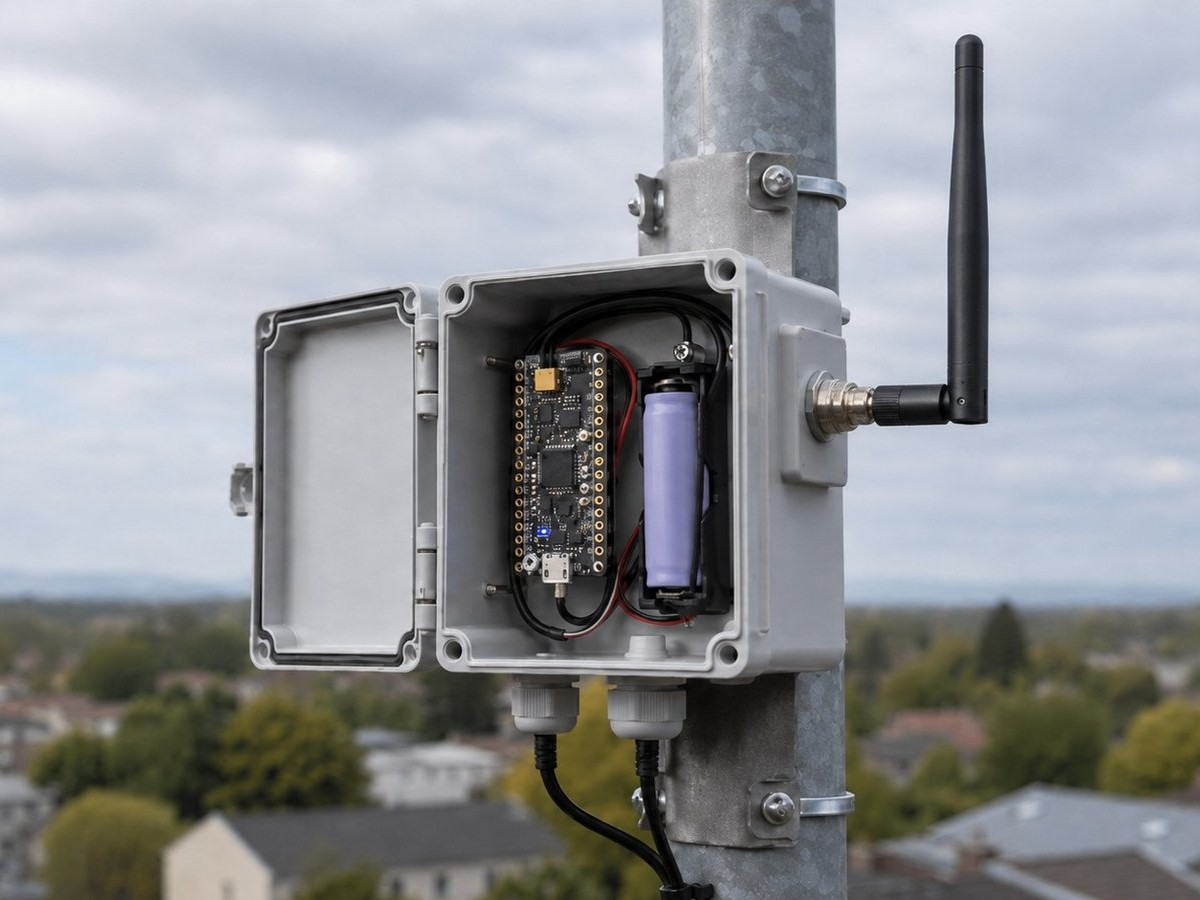
\includegraphics[width=0.75\linewidth]{images/repeater.jpg}
  \caption{outdoor node \cite{repeater-image}}
  \label{abb:node}
\end{figure}

Figure \ref{abb:node} is a simple yet perfectly usable example of a Heltec V3 board with a battery and an omnidirectional antenna.